Between September 4 and 10, 2017, there was a sudden increase in solar activity when Active Region 12673 produced four X-class flares, including the two strongest flares of Solar Cycle 24 (X9.3 on September 6 and X8.2 on September 10).
These solar events, associated with the release of energetic particles (\acp{SEP}) as well as the eruption of multiple fast \acp{CME}, caused a \ac{GLE} of energetic particles on the surface of Earth (\ac{GLE} \# 72 in the \ac{GLE} database at \url{https://gle.oulu.fi/}) as well as on Mars, making it the first \ac{GLE} observed simultaneously on the surface of two different planets.
This \ac{SEP} event was very widespread (Earth and Mars had a longitudinal separation of $\sim$\SI{155}{\degree} at that time) and the largest GLE seen on the surface of Mars with \ac{MSL}/\ac{RAD} so far.
These major events have been studied in great detail, many of the articles concerning these events can be found in the special issues of \citet{SpaceWeather-2018-special-issue-September-event} as well as \citet{GRL-2018-special-issue-September-event}, where the latter is focusing on its impact on Mars.

While the September 6 flare was a stronger event, the \acp{SEP} associated with the later September 10 flare is the one that was mainly seen at Earth and Mars, due to the better magnetic connection. Three CMEs also erupted on September 9 and 10 in similar directions ($\sim$\SI{115}{\degree} in \ac{HEE} coordinates), the last one with an extremely high speed of more than \SI{2600}{\kilo\meter\per\second}. This fast and wide CME quickly merged with the two previous ones and formed an intense interplanetary shock, propagated outward and was observed \textit{in situ} at both Earth and Mars on September 12 and 13, respectively. While the \ac{SEP} event at Mars was still in its declining phase, the shock arrival caused an intense \ac{FD} at Mars with an amplitude of \SI{15}{\percent}, the largest \ac{FD} seen by \ac{RAD} to date. This decrease below the pre-\ac{SEP} levels was sustained over 5 days and then gradually recovered over the course of several weeks.

The following two articles \citep{Zeitlin-2018,Guo-2018} study the effects of the September 10 events on Mars as measured by \ac{MSL}/\ac{RAD} and explain these observations by modeling the \ac{SEP} event and the three \acp{CME}. \citet{Zeitlin-2018} report the dosimetric quantities on the Martian surface, emphasizing that the increased dose and dose equivalent rates during the \ac{GLE} on Mars are almost canceled out by the long-lasting \ac{FD} following it. Thus, in the case of a long-stay mission scenario, the increased radiation exposure due to the September event would have been insignificant for astronauts on Mars despite the 2- to 3-fold increase during the peak of the \ac{SEP} event. However, as Mars was not particularly well connected to the active region, the impact of the \ac{SEP} event could have been much larger, so this conclusion should not be generalized to all major solar events at Mars. In \citet{Guo-2018}, the propagation of the 3 \acp{ICME} towards Earth and Mars is studied in more detail. The initial parameters of the \acp{CME} close to the Sun are reconstructed using \ac{GCS} fitting, and then the kinematics of the propagation are calculated using the empirical \ac{DBM} \citep{Vrsnak-2007,Vrsnak-2013}. This is one of the first instances where \ac{DBM} is used to predict the merging of multiple \acp{ICME} --- for this process, a simple conservation of momentum is assumed, and with a sensible choice of the drag parameter $\gamma$, it fits the observed arrival times at Earth and Mars. The results are also compared to more sophisticated \ac{MHD} simulations performed for the same event.

\newpage

The following article is reproduced from \textcite{Zeitlin-2018} with permission from Geophysical Research Letters, \copyright American Geophysical Union:\\

\pubcite{Zeitlin-2018}
\hfill Own contribution: 10\%

\newpage
\newcounter{includepdfpageZeitlinEighteen}

\addtocounter{section}{1}
\setcounter{subsection}{1} 
\phantomsection
\addcontentsline{toc}{section}{\arabic{chapter}.\arabic{section} Analysis of the radiation hazard observed by RAD on the surface of Mars during the September 2017 solar particle event (Publication GRL 2018)}
%
\phantomsection
\addcontentsline{toc}{subsection}{\arabic{chapter}.\arabic{section}.\arabic{subsection} Introduction}
\label{sec:paper_zeitlin2018}
%
\addtocounter{subsection}{1} 
\phantomsection
\addcontentsline{toc}{subsection}{\arabic{chapter}.\arabic{section}.\arabic{subsection} Triggering and Data Acquisition}
%
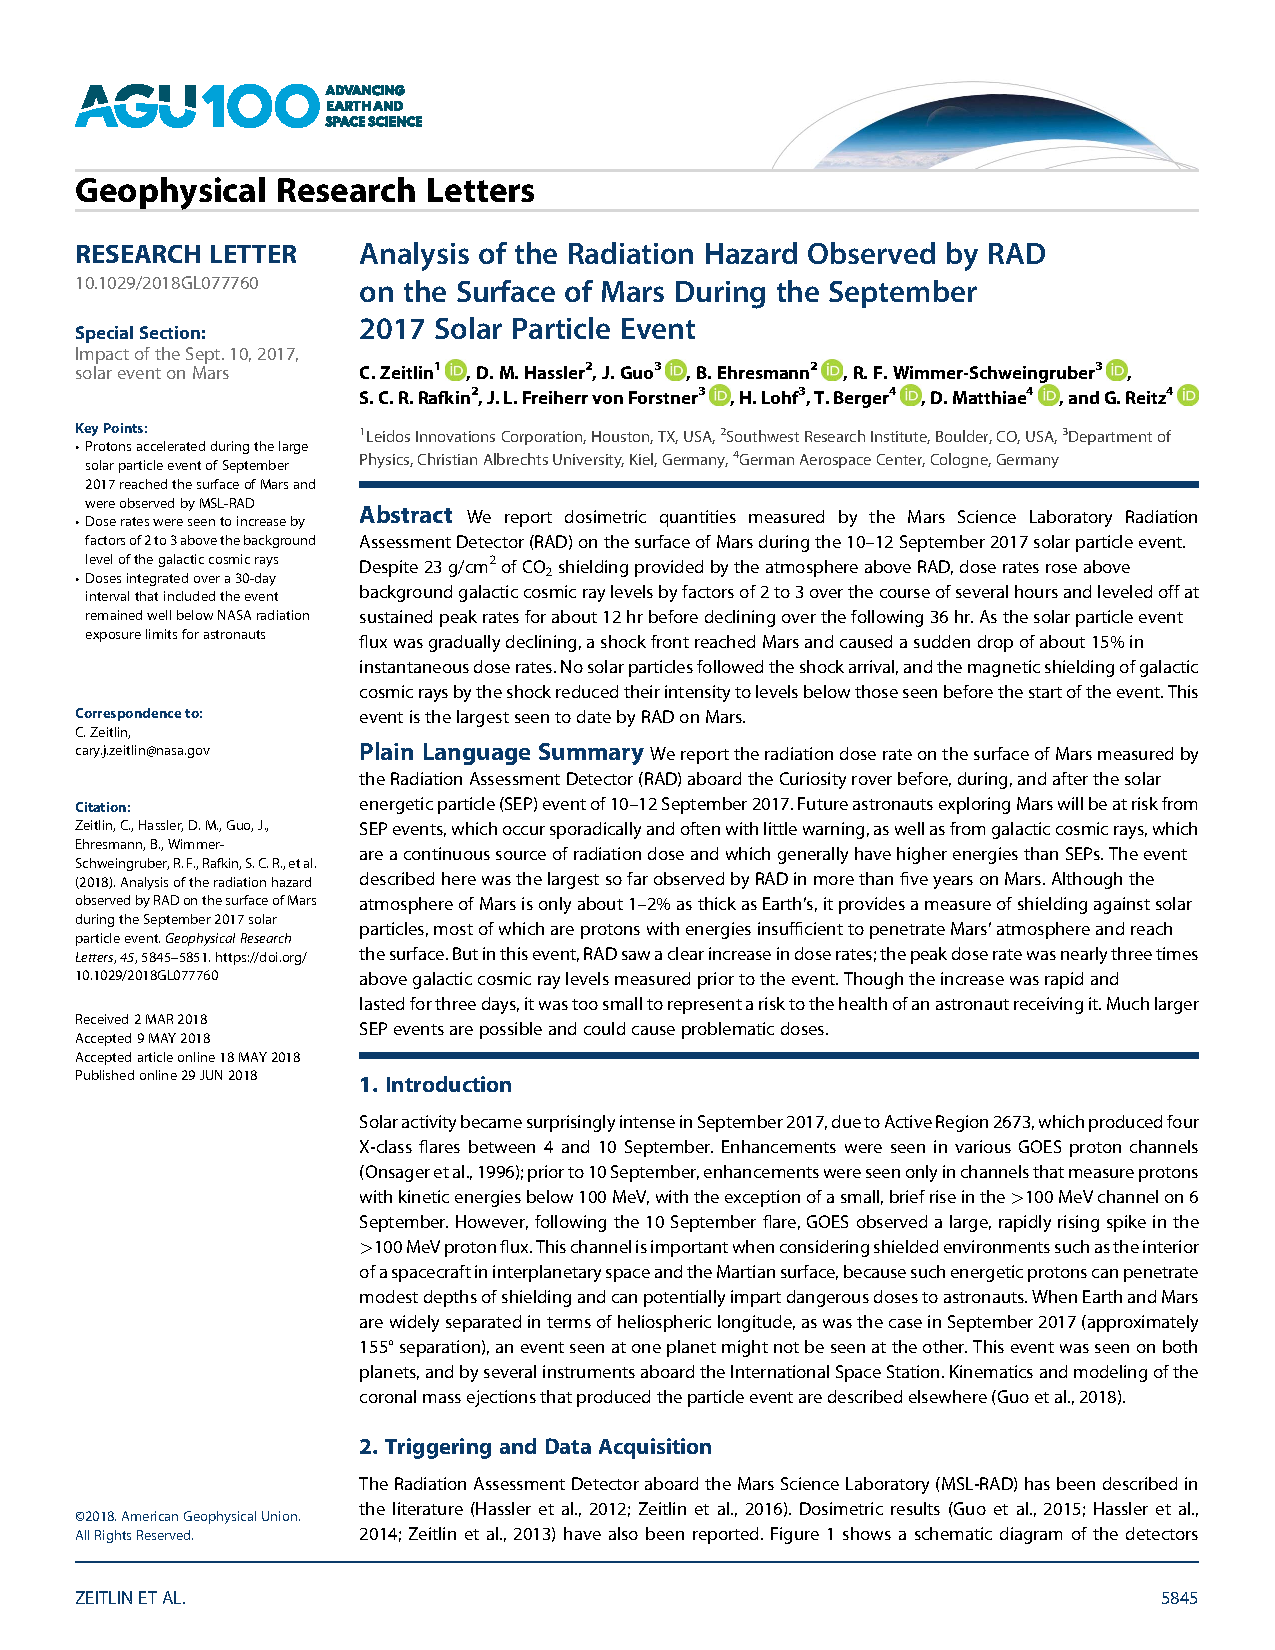
\includepdf[pages={1}, link, linkname=paper_zeitlin2018, scale=.95, pagecommand={\refstepcounter{includepdfpageZeitlinEighteen}\label{paper_zeitlin2018.\theincludepdfpageZeitlinEighteen}}]{publications/Zeitlin_et_al-2018-Geophysical_Research_Letters}
%
\addtocounter{subsection}{1} 
\phantomsection
\addcontentsline{toc}{subsection}{\arabic{chapter}.\arabic{section}.\arabic{subsection} Results}
\includepdf[pages={2-5}, link, linkname=paper_zeitlin2018, scale=.95, pagecommand={\refstepcounter{includepdfpageZeitlinEighteen}\label{paper_zeitlin2018.\theincludepdfpageZeitlinEighteen}}]{publications/Zeitlin_et_al-2018-Geophysical_Research_Letters}
%
\addtocounter{subsection}{1} 
\phantomsection
\addcontentsline{toc}{subsection}{\arabic{chapter}.\arabic{section}.\arabic{subsection} Conclusions}
\includepdf[pages={6}, link, linkname=paper_zeitlin2018, scale=.95, pagecommand={\refstepcounter{includepdfpageZeitlinEighteen}\label{paper_zeitlin2018.\theincludepdfpageZeitlinEighteen}}]{publications/Zeitlin_et_al-2018-Geophysical_Research_Letters}
%
\addtocounter{subsection}{1} 
\phantomsection
\addcontentsline{toc}{subsection}{\arabic{chapter}.\arabic{section}.\arabic{subsection} References}
\includepdf[pages={7}, link, linkname=paper_zeitlin2018, scale=.95, pagecommand={\refstepcounter{includepdfpageZeitlinEighteen}\label{paper_zeitlin2018.\theincludepdfpageZeitlinEighteen}}]{publications/Zeitlin_et_al-2018-Geophysical_Research_Letters}
\newpage

The following article is reproduced from \textcite{Guo-2018} with permission from Space Weather, \copyright American Geophysical Union:\\

\noindent
\pubcite{Guo-2018}
\hfill Own contribution: 10\%

\newpage
\newcounter{includepdfpageGuoEighteen}

\addtocounter{section}{1}
\setcounter{subsection}{1} 
\phantomsection
\addcontentsline{toc}{section}{\arabic{chapter}.\arabic{section} Modeling the Evolution and Propagation of 10 September 2017 CMEs and SEPs Arriving at Mars Constrained by Remote Sensing and In Situ Measurement (Publication Space Weather 2018)}
%
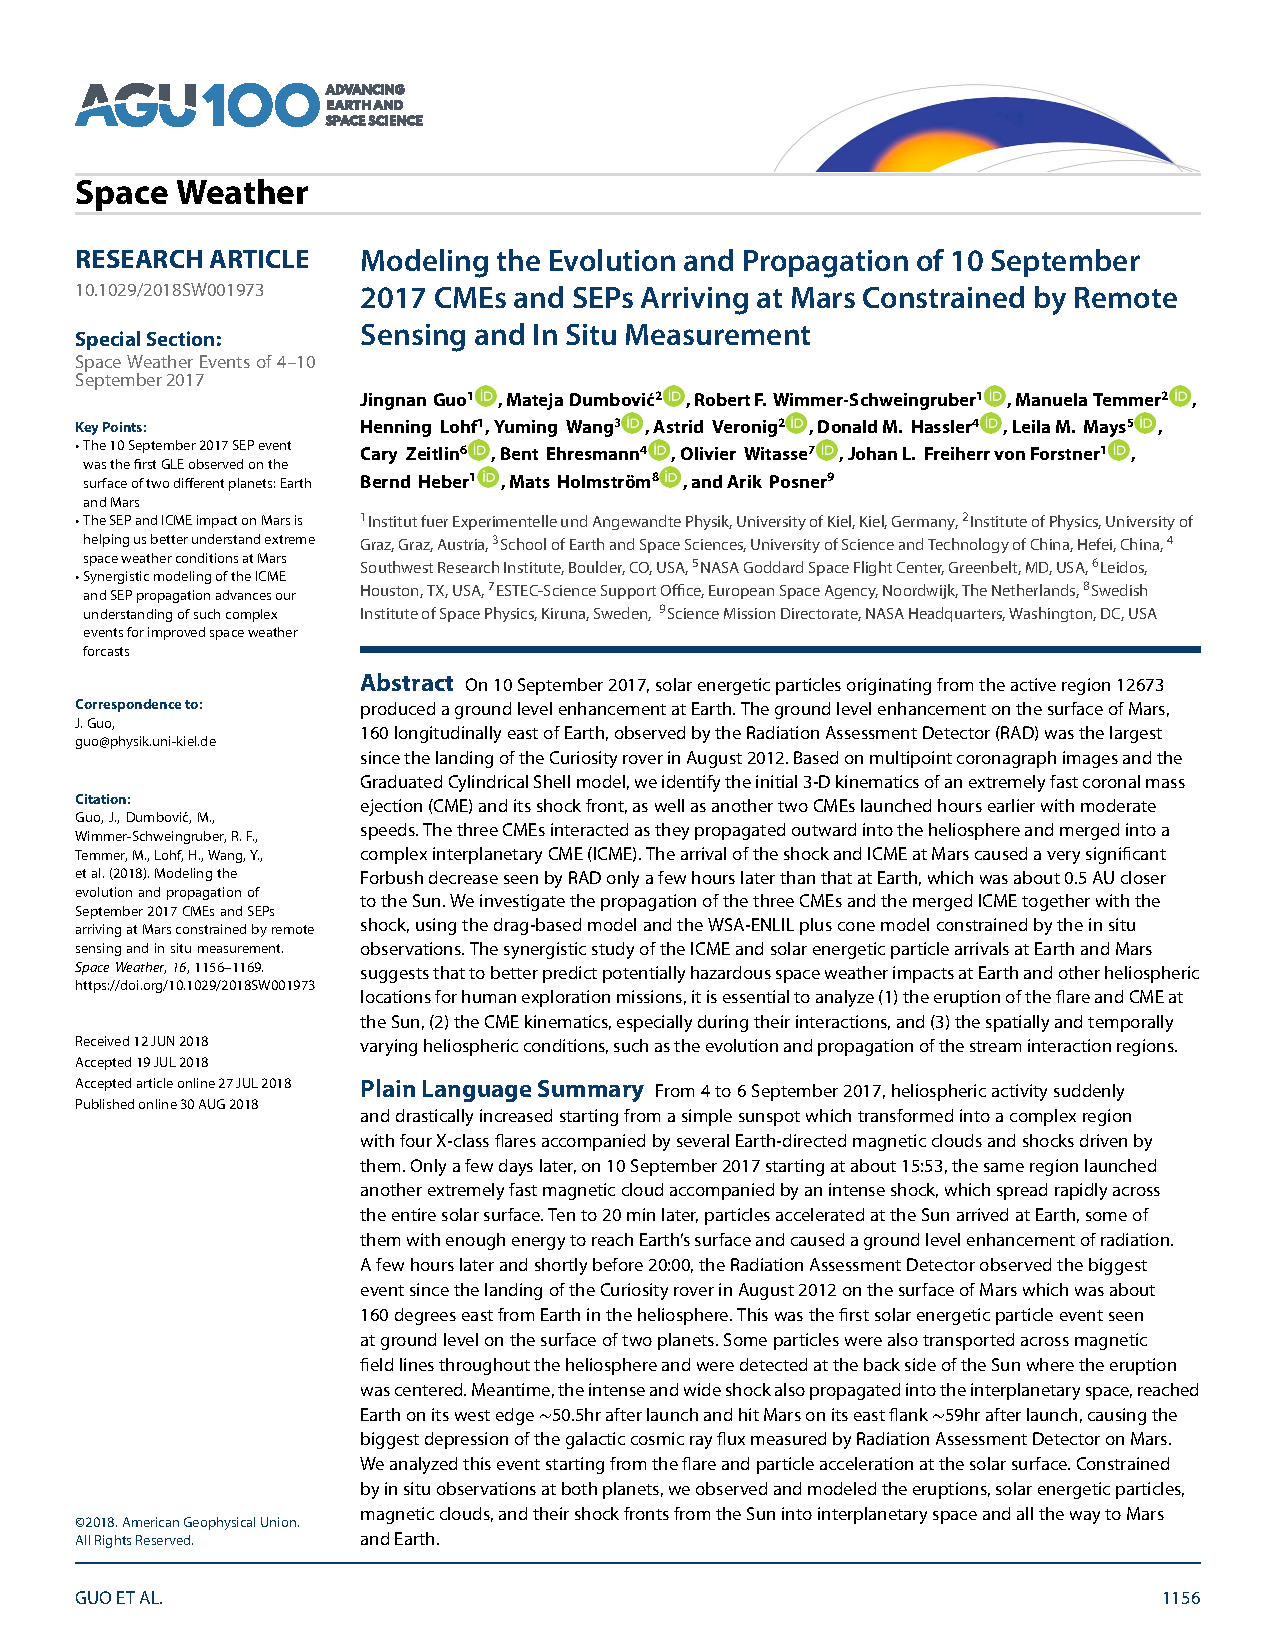
\includepdf[pages={1}, link, linkname=paper_guo2018, scale=.95, pagecommand={\refstepcounter{includepdfpageGuoEighteen}\label{paper_guo2018.\theincludepdfpageGuoEighteen}}]{publications/Guo_et_al-2018-Space_Weather}
%
\phantomsection
\addcontentsline{toc}{subsection}{\arabic{chapter}.\arabic{section}.\arabic{subsection} The Flare, CMEs, and GLE 72: Close to the Sun}
\label{sec:paper_guo2018}
%
\includepdf[pages={2-4}, link, linkname=paper_guo2018, scale=.95, pagecommand={\refstepcounter{includepdfpageGuoEighteen}\label{paper_guo2018.\theincludepdfpageGuoEighteen}}]{publications/Guo_et_al-2018-Space_Weather}
%
\addtocounter{subsection}{1} 
\phantomsection
\addcontentsline{toc}{subsection}{\arabic{chapter}.\arabic{section}.\arabic{subsection} The Interplanetary Trajectory and Interaction of Three CMEs Modeled by the DBM}
\includepdf[pages={5-6}, link, linkname=paper_guo2018, scale=.95, pagecommand={\refstepcounter{includepdfpageGuoEighteen}\label{paper_guo2018.\theincludepdfpageGuoEighteen}}]{publications/Guo_et_al-2018-Space_Weather}
%
\addtocounter{subsection}{1} 
\phantomsection
\addcontentsline{toc}{subsection}{\arabic{chapter}.\arabic{section}.\arabic{subsection} Shock Kinematics and Propagation Toward Earth and Mars: Data-Constrained DBM}
\includepdf[pages={7}, link, linkname=paper_guo2018, scale=.95, pagecommand={\refstepcounter{includepdfpageGuoEighteen}\label{paper_guo2018.\theincludepdfpageGuoEighteen}}]{publications/Guo_et_al-2018-Space_Weather}
%
\addtocounter{subsection}{1} 
\phantomsection
\addcontentsline{toc}{subsection}{\arabic{chapter}.\arabic{section}.\arabic{subsection} The Shock and ICME Arrival at Mars and Earth: Modeled Results and In Situ Observations}
\includepdf[pages={8}, link, linkname=paper_guo2018, scale=.95, pagecommand={\refstepcounter{includepdfpageGuoEighteen}\label{paper_guo2018.\theincludepdfpageGuoEighteen}}]{publications/Guo_et_al-2018-Space_Weather}
%
\addtocounter{subsection}{1} 
\phantomsection
\addcontentsline{toc}{subsection}{\arabic{chapter}.\arabic{section}.\arabic{subsection} SEPs Arriving at Earth, Mars, and STA and the Indication of the Shockand Stream Interaction Region Propagation}
\includepdf[pages={9-10}, link, linkname=paper_guo2018, scale=.95, pagecommand={\refstepcounter{includepdfpageGuoEighteen}\label{paper_guo2018.\theincludepdfpageGuoEighteen}}]{publications/Guo_et_al-2018-Space_Weather}
%
\addtocounter{subsection}{1} 
\phantomsection
\addcontentsline{toc}{subsection}{\arabic{chapter}.\arabic{section}.\arabic{subsection} Summary and Conclusion}
\includepdf[pages={11}, link, linkname=paper_guo2018, scale=.95, pagecommand={\refstepcounter{includepdfpageGuoEighteen}\label{paper_guo2018.\theincludepdfpageGuoEighteen}}]{publications/Guo_et_al-2018-Space_Weather}
%
\addtocounter{subsection}{1} 
\phantomsection
\addcontentsline{toc}{subsection}{\arabic{chapter}.\arabic{section}.\arabic{subsection} Appendix A: References of the Measurements and Databases Employed in This Study}
\includepdf[pages={12}, link, linkname=paper_guo2018, scale=.95, pagecommand={\refstepcounter{includepdfpageGuoEighteen}\label{paper_guo2018.\theincludepdfpageGuoEighteen}}]{publications/Guo_et_al-2018-Space_Weather}
%
\addtocounter{subsection}{1} 
\phantomsection
\addcontentsline{toc}{subsection}{\arabic{chapter}.\arabic{section}.\arabic{subsection} References}
\includepdf[pages={13-14}, link, linkname=paper_guo2018, scale=.95, pagecommand={\refstepcounter{includepdfpageGuoEighteen}\label{paper_guo2018.\theincludepdfpageGuoEighteen}}]{publications/Guo_et_al-2018-Space_Weather}